\section{From Biophysics to Evolutionary Genetics: Statistical aspects of gene
regulation}

In this section we will be exploring with all the glorious details all the
derivations done by Michael Lassig in his beautiful review paper for BMC
Bioinformatics 2007.

\subsection{Biophysics of transcriptional regulation}
As an area of expertise in the lab, we are very familiar with the statistical
mechanics of gene regulation. The model we will use for this section has a list
of important assumptions that we will explicitly state:

(A) Given a transcription factor binding site of length $l$ with sequence
$\mathbf{a} = (a_1, a_2, \ldots, a_l)$, the binding energy can be assumed to be
a linear contribution of each base-pair, i.e.
\begin{equation}
  E(\mathbf{a}) = \sum_{i=1}^l \varepsilon_i (a_i),
\end{equation}
where $a_i \in \{A, G, C, T \}$.

(B) At each position there is a preferred base-pair $a_i^*$ such that
\begin{equation}
  \varepsilon_i (a_i^*) = \min_a \varepsilon_i(a).
\end{equation}
Therefore it is assumed that there is a unique {\it ground state} $\mathbf{a}^*
\equiv (a_1^*, a_2^*, \ldots, a_l^*)$ with minimum binding energy $E^* \equiv
E(\mathbf{a}^*)$.

(C) Mismatches cost energy differences of order $\varepsilon_i (a) -
\varepsilon_i (a_i^*) \sim 1-3 \; k_BT$.

We can make an order of magnitude estimate assuming a two-state system in which
a position has either the optimal base-pair $a_i^*$ or not, i.e.
\begin{equation}
\varepsilon_i (a) - \varepsilon_i (a_i^*) =
\begin{cases}
  \varepsilon & \text{if } a \neq a_i^*\\
  0 & \text{otherwise},
\end{cases}
\end{equation}
with $\varepsilon \sim 1 \; k_BT$. This approximation allows us to define the
binding energy of a sequence a s a function of the Hamming distance
$d(\mathbf{a}, \mathbf{a^*})$, i.e. the number of base-pair mismatches between
sequences,
\begin{equation}
  E(\mathbf{a}) = E^* + \varepsilon \cdot d(\mathbf{a}, \mathbf{a^*}).
\end{equation}

\fref[fig_tf_binding_ecoli](a) shows the energy distribution for a proposition
weight matrix (PMW) of {\it CRP} along the genome. As we can note the energies
seem to be randomly distributed. We can bin the energy as shown in
\fref[fig_tf_binding_ecoli](b). In the limit of large number of positions by the
law of large numbers we expect the distribution of the energies to be Gaussian.
We can compute the mean and variance of this expected Gaussian distribution by
scrambling the genome and computing the resulting binding energies.
\fref[fig_tf_binding_ecoli](b) shows this prediction align the actual genomic
data. It can be seen that for the most part the genome is indeed randomly
distributed. But, \manuelComment{as done by Lassig in a very confusing way}, we
can zoom into the low energy tail to find that there are several low energy
sequences that are overrepresented in the genome that might be there not by
chance.

\begin{figure}[h!]
	\centering 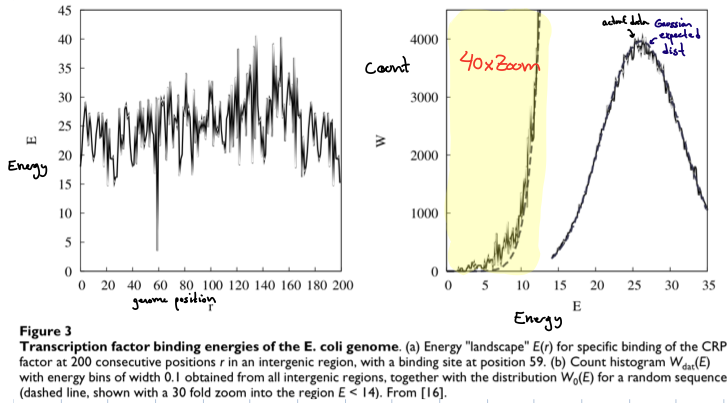
\includegraphics[scale=0.5]{../fig/lassig_2007/fig3.png}
	\caption{fig3}
  \label{fig_tf_binding_ecoli}
\end{figure}

\subsection{Thermodynamics of transcription factor binding}
\manuelComment{This section I don't feel is necessary in this document since
we are extremely familiar with that theory and my work is plagued with repeated
instances of this theory.}

\subsection{Sensitivity and genomic design of regulation}
Lassig goes into a very interesting and clever series of back-of-the-envelope
calculations about the design of regulatory binding sites given the physics of
transcription factor binding. The beautiful thing about these calculations is
that the numbers that come out are in perfect agreement with the inferred
binding energies for the {\it lac} repressor that we have always used. Let's go
through each of these calculations:

a) In a genome of length $\Nns \sim 5\times 10^6$ there must be at least one
{\it minimum energy} binding sites. If the genome was completely random
otherwise that would imply that the probability of finding the site would be
given by
\begin{equation}
  P(\mathbf{a}^*) = \prod_{i=1}^l P(a_i^*) = \left( {1 \over 4} \right)^l.
\end{equation}

The expected number of binding sites would then be constrained by
\begin{equation}
  \left\langle \text{\# binding sites} \right\rangle = \Nns P(\mathbf{a}^*)
   = \Nns \left( {1 \over 4} \right)^l \leq 1.
\end{equation}

Solving for the length of the binding site $l$ we find
\begin{align}
  \Nns &\leq 4^l\\
  \log \Nns &\leq l \log 4,
\end{align}
therefore
\begin{equation}
  l \geq {\log \Nns \over \log 4} \sim 10.
\end{equation}

b) If for a binding site of length $l$ there are $l$ possible sub-optimal
binding sites with Hamming distance 1, these sites should \textbf{not} suppress
binding to the optimal binding site. What this means is that it should hold
true that
\begin{equation}
  e^{-\beta E^*} \geq l e^{-\beta (E^* + \varepsilon)}.
\end{equation}
Solving for the energy difference $\varepsilon$ we find
\begin{align}
  -\beta E^* \leq \ln (l) - \beta (E^* + \varepsilon)\\
  \ln (l) \leq \beta \varepsilon \sim 2-3.
\end{align}
This implies that each base-pair should contribute with $\sim 2-3 \; k_BT$.

c) Finally the entirety of the {\it background genome} should not suppress
binding to the optimal binding site. Since we defined $E^*$ with respect to the
binding to the non-specific background it must hold true that
\begin{equation}
  e^{-\beta E^*} \geq \Nns e^{-\beta E_{NS}} = \Nns,
\end{equation}
since $E_{NS} = 0$ by definition.
This means that
\begin{equation}
  -\beta E^* \geq \log \Nns \sim 15.
\end{equation}
So the binding energy should be of order $-15 \; k_BT$ which is in perfect
agreement with the {\it lac} repressor.

\subsubsection{Programmability and evolvability of regulatory networks.}
In this section Lassig discusses very interesting points about the competition
between strong binding and evolvability.

If the cell wants to have a very specific binding of a transcription factor to
its corresponding functional binding site, the concept of {\it differential
programmability} would favor complicated molecular structures with long binding
sites to achieve large binding energies. However this competes with the {\it
evolvability} of the system via stochastic mutations.

Given the order-of-magnitude calculations in the previous section it seems that
indeed for the prokaryote case the gene regulatory machinery has almost single-
molecule sensitivity. This may result from a compromise between programmability
and evolvability, i.e. "binding sites are complicated enough to work."

\subsection{Bioinformatics of regulatory DNA.}
Lassig has come with a couple of methods to infer functional regulatory DNA that
takes into account the evolutionary history of the sequence. In this section we
will go through the logic of how to make these inferences.

\subsubsection{Markov model for background sequence}

Assuming that the genome is a Markov sequence with uniform probability for each
of the four nucleotides $P_o(a) = 1/4$, $a \in \{A, G, C, T \}$, we have that a
sequence $\mathbf{a}$ of length $k$ has a probability of occurring of the form
\begin{equation}
  P_o(\mathbf{a}) \prod_{i=1}^k P_o(a_i).
\end{equation}

Under the assumption that each base-pair contributes linearly to the total
binding site energy we can project the probability of sequences to the
\begin{equation}
  P_o(E) = \sum_{\mathbf{a}} P_o(\mathbf{a}) \delta(E - E(\mathbf{a})),
\end{equation}
where $\delta(x)$ is the delta function. What this equation syas is that the
probability of finding a sequence with binding energy $E$ is given by the sum
over all possible sequences, where the delta function guarantees that only the
sequences that happen to have the desired binding energy will contribute to the
sum. For example if only one sequence happened to have that specific energy, we
would sum over all possible sequences, but they would all be zero except for the
single sequence that maps to the desired energy. \fref[fig_tf_binding_ecoli](B)
shows that this model is very good at describing the genome.

\subsubsection{Probabilistic model for funcitonal sites.}

We can assume that the sequences $\mathbf{a} = (a_1, \ldots, a_l)$ on a binding
site are drawn from a different distribution $Q(\mathbf{a})$. We can then write
this distribution in terms of the non-specific distribution $P_o(\mathbf{a})$ as
\begin{equation}
  Q(\mathbf{a}) = P_o(\mathbf{a}) e^{S(\mathbf{a})},
\end{equation}
where $S(\mathbf{a})$ is called the {\it relative log-likelihood score} of the
distributions $P_o(\mathbf{a})$ and $Q(\mathbf{a})$. This quantity will be shown
to have an ipmortant evolutionary meaning, but for now we can trivially see that
this should be of the form
\begin{equation}
  S(\mathbf{a}) = \log \left( {Q(\mathbf{a}) \over P_o(\mathbf{a})} \right).
\end{equation}

For a single base-pair within the binding site we have that the probability of
a particular base $q_i(a)$, $i \in \{1, 2, \ldots, l\}$, $a \in \{A, G, C, T \}$
can be obtained by marginalizing the distribution $Q(\mathbf{a})$ as
\begin{equation}
  q_i(a) = \sum_{a_1} \sum_{a_2} \cdots \sum_{a_{i-1}}\sum_{a_{i+1}}
  \cdots \sum_{a_l} Q(a_1, a_2, \ldots, a_{i-1}, a_{i}, a_{i+1}, \ldots, a_l),
\end{equation}
or written in a compact form
\begin{equation}
  q_i(a) = \sum_{a_j \neq a_i} Q(\mathbf{a}).
\end{equation}
It is the set of these marginal distributions $q_i(a)$ that form the so-called
position weight matrix. If the score function $S(\mathbf{a})$ is additive in the
base-pair positions, i.e. $S(\mathbf{a}) = \sum_{i=1}^l s_i(a)$, then the
distribution $Q(\mathbf{a})$ has a factorized form
\begin{equation}
  Q(\mathbf{a}) = \prod_{i=1}^l q_i(a),
\end{equation}
with
\begin{equation}
  q_i(a) = P_o(a)\exp\left[ s_i(a) \right]
\end{equation}

We can again map the distribution into energies as
\begin{equation}
  Q(E) = \sum_{\mathbf{a}} Q(\mathbf{a}) \delta (E - E(\mathbf{a})),
\end{equation}
as well as the score function
\begin{equation}
  S(E) = \sum_{\mathbf{a}} S(\mathbf{a}) \delta (E - E(\mathbf{a})).
\end{equation}
Hence we can write
\begin{equation}
  Q(E) = P_o(E)\exp\left[ S(E) \right]
\end{equation}

\subsubsection{Bayesian model for genomic loci.}

We can now assume that the functional binding sites are distributed along the
genome with a small probability of occurring, $\lambda$. This allows us to
combine both distributions $P_o(\mathbf{a})$ and $Q(\mathbf{a})$ into something
called a Hidden Markov Model for a genomic sequence as
\begin{equation}
  W(\mathbf{a}) = \lambda Q(\mathbf{a}) + (1 - \lambda) P_o(\mathbf{a}),
\end{equation}
where $\lambda$ is known as the hidden variable.

The output of this model consists of pairs $(m, \mathbf{a})$ where first a
sequence is assigned as non-functional $(m=0)$ with probability $(1 - \lambda)$
or functional $(m=1)$ with probability $\lambda$. Based on this result the
sequence $\mathbf{a}$ is drawn out of $P_o(\mathbf{a})$ or $Q(\mathbf{a})$.
However we only have access to sequences $\mathbf{a}$ as data. The hidden
variable $m$ can be inferred from data using Bayes theorem as
\begin{equation}
  P(m \mid \mathbf{a}) = {P(\mathbf{a} \mid m) P(m) \over P(\mathbf{a})}.
\end{equation}
This an be rewritten as
\begin{equation}
  P(m \mid \mathbf{a}) = {P(\mathbf{a} \mid m) P(m) \over
  \sum_{m=0}^1 P(\mathbf{a} \mid m) P(m)}.
\end{equation}

This means that the probability of a given sequence $\mathbf{a}$ being
functional $\rho_f(\mathbf{a}) \equiv P(m=1\mid \mathbf{a})$ is given by
\begin{equation}
  \rho_f(\mathbf{a}) = {P(\mathbf{a} \mid m=1) P(m=1) \over
  P(\mathbf{a} \mid m=1) P(m=1) + P(\mathbf{a} \mid m=0) P(m=0)}.
\end{equation}
Writing this in terms of our distributions for specific and non-specific sites
gives
\begin{equation}
  \rho_f(\mathbf{a}) = {Q(\mathbf{a}) \cdot \lambda \over
  Q(\mathbf{a}) \cdot \lambda + P_o(\mathbf{a}) \cdot (1 - \lambda)}
\end{equation}

Rearranging terms we have
\begin{equation}
  \rho_f(\mathbf{a}) = {1 \over 1 + {(1 - \lambda) \over \lambda}
  {P_o(\mathbf{a}) \over Q(\mathbf{a})}}.
\end{equation}
Using the score function $S(\mathbf{a})$ gives
\begin{align}
  \rho_f(\mathbf{a}) &= {1  \over 1 + {(1 - \lambda) \over \lambda}
  \exp\left[ - S(\mathbf{a}) \right]},\\
  &= {1  \over 1 + \exp\left[ - S(\mathbf{a}) + \ln {(1 - \lambda) \over
  \lambda} \right]}.
\end{align}
When written in this form the function takes the form of a Fermi function with
threshold value $S(\mathbf{a}) = \ln {(1 - \lambda) \over \lambda}$ separating
the sequences likely to be functional from the non-functional ones.

This Bayesian model can again be projected onto energies
\begin{equation}
  W(E) = \lambda Q(E) + (1 - \lambda) P_o(E).
\end{equation}

\fref[fig_bayesian_dna] shows the application of this model to {\it CRP} on the
{\it E. coli} genome. This model seems to account for the data displayed.

\begin{figure}[h!]
	\centering 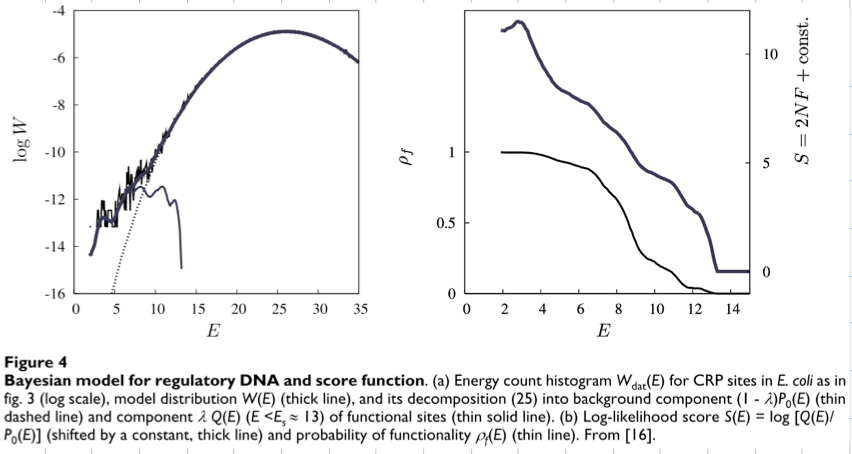
\includegraphics[scale=0.5]{../fig/lassig_2007/fig4.png}
	\caption{fig3}
  \label{fig_bayesian_dna}
\end{figure}

\subsection{Evolution of regulatory DNA.}

In this section of the paper Lassig explores the application of population
genetics ideas to the evolution of regulatory sequences. In principle the
statistical picture developed so far lacks two things:
\begin{enumerate}
  \item the specific functionality that binding provides to the transcription
  factor, since the PWM formalism doesn't care about the functionality of
  binding
  \item The sense of time and dynamics as dictated by the evolutionary history
  of these sequences. It is important to highlight that functional loci evolve
  fundamentally different from background sequences since these functional loci
  are subject to natural selection.
\end{enumerate}
It is therefore why at this point we will integrate the biophysics of binding
with the evolution of functional sequences.

\subsubsection{Deterministic population dynamics and fitness.}

Let us begin with a deterministic approach. We will be describing the evolution
of a population with different genotypes for the binding sequence. We assume
that the relevant phenotype is the binding energy for which we can use the PWM
approach to map form genotype to phenotype. For our discussion we will imagine
a population of asexual organisms in which recombination is non-existent.
The dynamics of this population can be written as
\begin{equation}
  \dt{N_\bb{a}(t)} = F_\bb{a}(t) \cdot N_\bb{a}(t),
\end{equation}
where $F_\bb{a}(t)$ is the Malthusian fitness for sequence $\bb{a}$ at time $t$.
For simplicity let's focus on two genotypes: $\bb{a} = (a_1, a_2, \ldots, a_l)$
and $\bb{b} = (b_1, b_2, \ldots, b_l)$. We can write a similar equation for
genotype $\bb{b}$. The total number of organisms at any time is then given by
\begin{equation}
  N_\tot(t) \equiv N_\bb{a}(t) + N_\bb{b}(t).
\end{equation}
Let's assume we are interested in tracking the relative abundance of $\bb{b}$.
We then define $x(t) \equiv {N_\bb{b}(t) \over N_\tot(t)}$. We can write the
dynamics for both $N_\tot(t)$ and $x(t)$ as
\begin{align}
\dt{N_\tot} &= \bar{F} N_\tot(t),\\
&= F_\bb{a}(t) N_\bb{a}(t) + F_\bb{b}(t) N_\bb{b}(t),\\
&= N_\tot(t) \left[ F_\bb{a}(t) (1 - x(t)) + F_\bb{b} x(t) \right],
\end{align}
and
\begin{equation}
  \dt{x} = {d \over dt} \left( {N_\bb{b}(t) \over N_\tot(t)} \right)
  = {\dot{N}_\bb{b}(t) N_\tot(t) - N_\bb{b}(t) \dot{N}_\tot(t) \over
     N_\tot(t)^2},
\end{equation}
where $\dot{f} \equiv df/dt$. If we substitute the equations for the time
derivatives of the number of organisms we have
\begin{equation}
  \dt{x} = {F_\bb{b}(t) N_\bb{b}(t) N_\tot(t) \over N_\tot(t)^2} -
  {N_\bb{b}(t) \left[ F_\bb{a}(t)N_\bb{a}(t) + F_\bb{b}(t)N_\bb{b}(t) \right]
  \over N_\tot(t)^2}.
\end{equation}
This can be further simplified to
\begin{align}
  \dt{x} &= F_\bb{b}(t) \overbrace{N_\bb{b}(t) \over N_\tot(t)}^{x(t)} -
  \overbrace{N_\bb{b}(t) \over N_\tot(t)}^{x(t)}
  \left[ F_\bb{a}(t) (1 - x(t)) + F_\bb{b}(t) x(t) \right],\\
  &= x(t) \left[ F_\bb{b}(t) (1 - x(t)) - F_\bb{a}(t) (1 - x(t)) \right].
\end{align}

Therefore the time derivative of the relative abundance of the genotype $\bb{b}$
can be simply written as
\begin{equation}
  \dt{x} = \DF(t) x(t) (1 - x(t)),
\end{equation}
where $\DF \equiv F_\bb{b}(t) - F_\bb{a}(t)$.

If we assume $\DF(t)$ to be independent of time we can solve $\dot x(t)$ as
\begin{equation}
  \dt{x} = \DF x(t) (1 - x(t)) = \DF \left( x(t) - x(t)^2 \right),
\end{equation}
which is a first order linear differential equation that can be solved by the
method of separation of variables as
\begin{equation}
  \int {dx \over x (1 - x)} = \DF \int dt.
\end{equation}
Focusing on the left-hand side we can use partial fraction decomposition as
\begin{equation}
  {A \over x} + {B \over 1 - x} = {1 \over x (1 - x)}.
\end{equation}
This implies that for $x = 1$, $B = 1$ and for $x = 0$, $A = 1$. Therefore the
integral can be rewritten as
\begin{equation}
  \int {dx \over x (1 - x)} = \int {dx \over x} + \int {dx \over 1 - x}
  = \ln x - \ln (1 - x) + C.
\end{equation}

Therefore we have that
\begin{equation}
  \ln \left( {x \over 1 - x} \right) = \DF t + C.
\end{equation}
To remove the integration constant we can specify the initial condition
$x(0) = x_o$. With this we find that $C = \ln (x_o / 1 - x_o)$. Substituting
this and exponentiating both sides of the equation gives
\begin{equation}
  {x \over 1 - x} = e^{\DF t} \left( {x_o \over 1 - x_o } \right).
\end{equation}
Solving for $x$ we find
\begin{align}
  &x = e^{\DF t} \left( {x_o} \over 1 - x_o \right)(1 - x),\\
  \Rightarrow &x \left[ 1 + e^{\DF t} \left( {x_o} \over 1 - x_o \right) \right]
  = e^{\DF t} \left( {x_o \over 1 - x_o} \right),\\
  \Rightarrow &x \left[ 1 - x_o + e^{\DF t} x_o \right] = e^{\DF t} x_o.
\end{align}
Therefore the dynamics of the relative abundance of genotype $\bb{b}$ are given
by
\begin{equation}
  x(t) = {e^{\DF t} x_o \over 1 + x_o \left( e^{\DF t} - 1 \right)}.
\end{equation}

Given the equation for $\dot{x}(t)$ we can say something about the dynamics and
the stable points. Since we have that
\begin{equation}
  \dt{x} = \DF (x(t) - x(t)^2),
\end{equation}
we can plot the linear and the quadratic term to see the stable points as shown
in \fref[fig_phase_portrait]. For $\DF > 0$ we have two stable points, one
attractor at $x = 1$ and one repeller at $x = 0$. The opposite is true for the
case where $\DF < 0$. Finally from the equation we can see that the approach to
stationary phase takes a characteristic time of order $\tau \sim {1 \over \DF}$.

\begin{figure}[h!]
	\centering 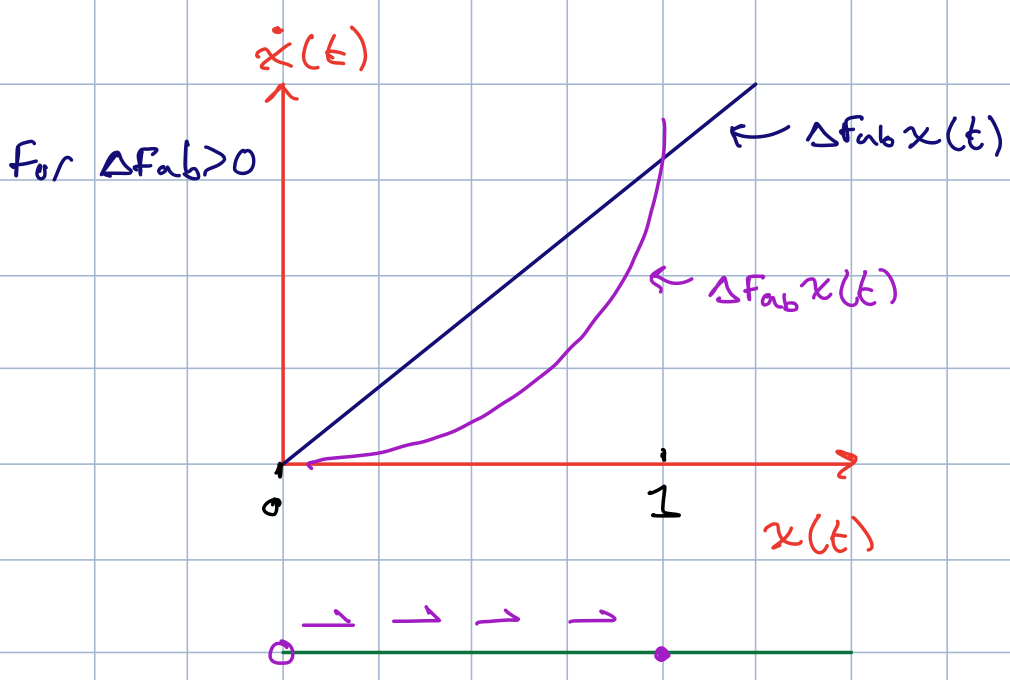
\includegraphics[scale=0.5]{../fig/lassig_2007/phase_portrait.png}
	\caption{fig3}
  \label{fig_phase_portrait}
\end{figure}

This is not other than a simple version of Fisher's fundamental theorem of
natural selection: Any population with initially coexisting phenotype of
different fitness will evolve towards a state in which only the fittest
phenotype is present. There is a very interesting paragraph on Lassig's paper
related to my ideas and projects. So it is worth quoting it here:
{\it Fisher's theorem seems to prove the popularized Darwinian notion of the
"survival of the fittest". However, it rests on very restrictive assumptions
that are never fulfilled in a natural population. The deterministic growth law
(32) neglects mutations and recombinations, as well as the reproductive
fluctuations present in any population due to its finite number of individuals.
These other evolutionary forces have to be incorporated in our theoretical
picture before we can even define fitness as a measurable quantity and before
the theory can address the important case of neutral evolution.}

\subsubsection{Stochastic dynamics and genetic drift.}

Using the stochastic processes formalism we will now incoorporate random
fluctuations in reproductive success of our modeled population. With a Langevin
dynamics framework we can write the growth law as
\begin{equation}
  \dt{N_\bb{a}} = F_\bb{a}(t) N_\bb{a}(t) + \chi_\bb{a}(t),
\end{equation}
where $\chi_\bb{a}(t)$ is the noise term in the growth. To make analytical
progress we define $\chi_\bb{a}$ to be Gaussian distributed with mean
\begin{equation}
  \moment{\chi_\bb{a}} = 0.
\end{equation}
The correlation function $\moment{\chi_\bb{a}(t) \chi_\bb{b}(t)}$ between
genotypes $\bb{a}$ and $\bb{b}$ is set to be
\begin{equation}
  \moment{\chi_\bb{a}(t) \chi_\bb{b}(t)} = N_\bb{a}(t)
                                           \delta(t - t') \delta_\bb{ab}.
\end{equation}
What this equation says is first of all that all genotypes noise is independent
of other genotypes via the delta function $\delta_\bb{ab}$ which is equal to one
if and only if $\bb{a} = \bb{b}$. Second of all this equation tells us that the
noise is completely uncorrelated over time; this is set by the delta function
$\delta(t - t')$ which is one only if $t' = t$. What that implies is that the
function will only be non-zero when evaluated as
\begin{equation}
  \moment{\chi_\bb{a}(t) \chi_\bb{a}(t)} = \moment{\chi_\bb{a}(t)^2} = N_\bb{a}.
\end{equation}
Since $\moment{\chi_\bb{a}(t)} = 0$, $\moment{\chi_\bb{a}(t)}^2$ is the variance
of the random noise which is set to be $N_\bb{a}(t)$ as for a Poisson process.
Note that formally $N_\bb{a}(t)$ must be interpreted as the {\it effective
population size} rather than the absolute population size.

If we project this stochastic growth to population fraction we find just as
before
\begin{equation}
  \dt{x} = \dt{}\left( {N_\bb{b}(t) \over N_\tot(t)} \right) =
  {\dot{N}_\bb{b}(t) N_\tot(t) - N_\bb{b}(t) \dot{N}_\tot(t) \over
     N_\tot(t)^2}.
\end{equation}

Substituting the definition of the time derivatives we find
\begin{equation}
  \dt{x} = {\left[ F_\bb{b}(t) N_\bb{b}(t) + \chi_\bb{b}(t)  \right] N_\tot(t)
  \over N_\tot(t)^2} -
  {N_\bb{b}(t)
  \left[ F_\bb{b}(t) N_\bb{b}(t) + \chi_\bb{b}(t) +
         F_\bb{a}(t) N_\bb{a}(t) + \chi_\bb{a}(t)\right] \over N_\tot(t)^2}.
\end{equation}
We now divide each term by $N_\tot(t)^2$, obtaining
\begin{equation}
  \dt{x} = F_\bb{b}(t)x(t) + {\chi_\bb{b}(t) \over N_\tot(t)} -
  x(t) \left[ F_\bb{b}(t)x(t) + {\chi_\bb{b}(t) \over N_\tot(t)} +
              F_\bb{a}(t)(1 - x(t)) + {\chi_\bb{a}(t) \over N_\tot(t)} \right].
\end{equation}
We can then factorize terms to obtain
\begin{equation}
  \dt{x} = \DF(t) x(t) (1 - x(t)) + {1 \over N_\tot(t)}
  \left( \chi_\bb{b}(t)(1 - x(t)) - \chi_\bb{a}(t) x(t) \right).
\end{equation}

We can cleverly transform the last terms if we note that
\begin{align}
  {\partial x \over \partial N_\bb{b}} &= {\partial \over \partial N_\bb{b}}
  \left( {N_\bb{b} \over N_\tot} \right), \\
  &= {1 \over N_\tot^2} \left[ 1 \cdot N_\tot - N_\bb{b} \cdot 1 \right],\\
  &= {1 \over N_\tot}(1 - x).
\end{align}
And similarly
\begin{align}
  {\partial x \over \partial N_\bb{a}} &= {\partial \over \partial N_\bb{a}}
  \left( {N_\bb{b} \over N_\tot} \right), \\
  &= {0 \over N_\tot^2} \left[ 1 \cdot N_\tot - N_\bb{b} \cdot 1 \right],\\
  &= - {x \over N_\tot}.
\end{align}
With this we can rewrite $\dot{x}(t)$ as
\begin{equation}
  \dt{x} = \DF(t) x(t) (1 - x(t)) + \overbrace{
  {\partial x \over \partial N_\bb{b}} \chi_\bb{b}(t) +
  {\partial x \over \partial N_\bb{a}} \chi_\bb{a}(t)
  }^{\chi_x(t)}.
\end{equation}
Since our definition of $\chi_x(t)$ involves a sum of Gaussian random variables
we know that $\chi_x(t)$ is Gaussian distributed itself. We can use two rules
about adding Gaussian random variables: If we add two Gaussian random variables
with mean $\mu_1$ and $\mu_2$ and variance $\sigma_1^2$ and $\sigma_2^2$, the
sum of these variables gives a variable of the form
\begin{equation}
  X_1 + X_2 \sim \mathcal{N}\left( \mu_1 + \mu_2,
                                   \sigma_1^2 + \sigma_2^2 \right).
\end{equation}
Also a linear transformation of a Gaussian random variable gives
\begin{equation}
  a + b \mathcal{N} \left( \mu, \sigma^2 \right) =
  \mathcal{N}(a + b \mu, b^2 \sigma^2).
\end{equation}

Using these rules we have that
\begin{align}
{(1 - x(t)) \over N_\tot(t)} \cdot \chi_\bb{b}(t) &=
{(1 - x(t)) \over N_\tot(t)} \cdot \mathcal{N}(0, N_\bb{b}(t)),\\
&= \mathcal{N}\left( 0, {(1 - x(t))^2 \over N_\tot(t)^2} N_\bb{b}(t) \right),\\
&= \mathcal{N}\left( 0, {(1 - x(t))^2 x(t) \over N_\tot(t)} \right).
\end{align}
Also
\begin{align}
  -{x(t) \over N_\tot(t)} \chi_\bb{a}(t) &=
  -{x(t) \over N_\tot(t)} \mathcal{N}\left( 0, N_\bb{a}(t) \right),\\
&= \mathcal{N}\left( 0, {x(t)^2 \over N_\tot(t)^2} N_\bb{a}(t) \right),\\
&= \mathcal{N}\left( 0, {x(t)^2 (1 - x(t)) \over N_\tot(t)} \right).
\end{align}

Since $\chi_x(t)$ is given by the sum of these random variables we have that
\begin{equation}
  \chi_x(t) \sim \mathcal{N}\left(0,  {(1 - x(t))^2 x(t) \over N_\tot(t)} +
   {x(t)^2 (1 - x(t)) \over N_\tot(t)} \right).
\end{equation}

Simplifying the variance we have
\begin{align}
  {(1 - x(t))^2 x(t) \over N_\tot(t)} + {x(t)^2 (1 - x(t)) \over N_\tot(t)} &=
  {x(t) - 2 x(t)^2 + x(t)^3 + x(t)^2 - x(t)^3 \over N_\tot(t)},\\
  &= {x(t) - x(t)^2 \over N_\tot(t)}, \\
  &= {x(t) (1 - x(t)) \over N_\tot(t)}.
\end{align}
Therefore $\chi_x$ is distributed as
\begin{equation}
  \chi_x(t) \sim \mathcal{N} \left( 0, {x(t) (1 - x(t)) \over N_\tot(t)}
  \right).
\end{equation}
This can be written in terms of the autocorrelation function as
\begin{equation}
  \moment{\chi_x(t) \chi_x(t')} = {x(1 - x) \over N_\tot} \delta(t - t'),
\end{equation}
where all we are saying is that the fractional noise $\chi_x$ is completely
random and is not correlated in time with itself.

\subsubsection{From Langevin dynamics to Fokker-Planck equations.}

\manuelComment{In a single statement with no derivation Lassig uses the
Langevin equation for the genotype fraction to derive a corresponding Fokker-
Planck equation. This is far from trivial and the derivation requires some
heavy machinery.}
The full derivation of the connection between Langevin dynamics and Fokker-
Planck formulation will be left for a separate set of notes \manuelComment(to
be written later on). for our purpose it suffices to say that from a Langevin
equation of the form
\begin{equation}
  \dt{x} = A(x, t) + B(x, t) \xi(t),
\end{equation}
where $A(x, t)$ is known as the drift or directional term and $B(x, t)$ is the
stochastic coefficient of the diffusion random term $\xi(t)$ with properties
\begin{equation}
  \moment{\xi(t)} = 0,
\end{equation}
and
\begin{equation}
  \moment{\xi(t) \xi(t')} = 2D \delta(t - t'),
\end{equation}
we have a corresponding Fokker-Planck equation of the form
\begin{equation}
  {\partial P \over \partial t} = - {\partial \over \partial x}
  \left\{ \left[ A(x, t) + D B(x, t) {\partial B(x, t) \over \partial x}
  \right] P \right\} +
  D {\partial^2 \over \partial x^2} \left\{ \left[ B(x, t)^2 \right] P \right\}.
\end{equation}

Let's now find the corresponding terms in our equation. We have that the
directional or drift term is given by
\begin{equation}
  A(x, t) = \DF(t) x(t) (1 - x(t)).
\end{equation}
For the diffusion term $\chi_x \sim \mathcal{N} \left( 0, x(1-x)/N_\tot \right)$
we will redefine it to be
\begin{equation}
  \chi_x = \left[ {x (1 - x) \over N_\tot} \right]^{1/2} \xi_x,
\end{equation}
where $\xi_x \sim \mathcal{N}(0, 1)$, so that the $x$ dependence of the variance
is sent to the $B(x, t)$ coefficient. With this we then have that
\begin{equation}
  B(x, t) = \left[ {x (1 - x) \over N_\tot} \right]^{1/2}.
\end{equation}
For simplicity from now on we won't make the time dependence explicit, such that
$x \equiv x(t)$, also we will simply write $N \equiv N_\tot(t)$.

Since we have $\moment{\xi_x(t) \xi_x(t't)} = \delta(t - t')$, it must be the
case that $D \equiv {1 \over 2}$. Let's now try to build the Fokker-Planck
equation
\begin{equation}
  {\partial P \over \partial t} = - {\partial \over \partial x}
  \left\{ \left[ \DF x (1 - x) +
  \textcolor{purple}{{1 \over 2} \left( {x (1 - x) \over N} \right)^{1/2}
  {\partial \over \partial x} \left( x (1 - x) \over N \right)^{1/2}}
  \right] P \right\} +
  {1 \over 2} {\partial^2 \over \partial x^2} \left[ {x (1 - x) \over N} P
  \right].
\end{equation}

This result is almost directly Lassig's and more correctly Kimura's formulation
of diffusion theory except for the second term highlighted in
\textcolor{purple}{red}. This term represents the {\it noise-induced drift} term
that I have personally never seen before. Let's epxlore this term a little bit
further by taking the derivative
\begin{align}
  -{\partial \over \partial x} \left\{ {1 \over 2}
  \left( {x (1 - x) \over N} \right)^{1/2}
  {\partial \over \partial x} \left( {x (1 - x) \over N} \right)^{1/2} P
  \right\} &=
  - {1 \over 2 N} {\partial \over \partial x} \left\{ [x (1 - x)]^{1/2}
  \left[ {1 \over 2} {{(1 - x) - x} \over [x (1 - x)]^{1/2}} \right] P
  \right\},\\
  &= -{1 \over 4 N} {\partial \over \partial x}\left\{ (1 - 2 x) P \right\}.
\end{align}
\manuelComment{I find this term quite interesting. My interpretation is the
following: The diffusion term ${1\over 2} \partial_{xx} x (1 - x) P$ has "no
sense of direction." The magnitude of the jump depends on where are you standing
on the real line, but it is equally likely to jump left or right. This can be
clearly seen if one takes the "spread the butter" approach. There is easy to
note that indeed the magnitude of the jump depends on where are you standing
in frequency space, but the magnitude applies to both directions left and right.
In the case of this directional term $- {1 \over 2} \partial x (1 - 2x) P$
breaks the symmetry of these jumps. The closer you get to 1 or 0, the more you
jump towards that direction. That is why at $x = {1 \over 2}$ this term
vanishes.}

The two versions of the Fokker-Planck equation are then:
\paragraph{Lassig / Kimura}
\begin{equation}
  {\partial P \over \partial t} = {1 \over 2N}
  {\partial^2 \over \partial x^2} \left[ x (1 - x) P \right] -
  \DF {\partial \over \partial x} \left[ x (1 - x)  \right]
\end{equation}

\paragraph{Complete equation}
\begin{equation}
  {\partial P \over \partial t} = {1 \over 2N}
  {\partial^2 \over \partial x^2} \left[ x (1 - x) P \right] -
  \DF {\partial \over \partial x} \left[ x (1 - x)  \right] -
  {1 \over 4N} {\partial \over \partial x} \left[ (1 - 2x) P \right].
\end{equation}

The steady-state solution of this Fokker-Planck equation is fo the form
\begin{equation}
  P(x) = {C \over V(x)} \exp \left\{ 2 \int dx {M(x) \over V(x)} \right\},
\end{equation}
where $M(x)$ includes all directional processes and $V(x)$ captures all
diffusive processes. For our specific equation we have
\begin{equation}
  M(x) = \DF x (1 - x) + \overbrace{{1 \over 4N} (1 - 2x)}^
  {\text{extra term from the noise-induced drift}},
\end{equation}
and
\begin{equation}
  V(x) = {1 \over N} x (1 - x).
\end{equation}

This means that the integral in the steady state solution takes the form
\begin{equation}
  \int dx {M(x) \over V(x)} = \int dx \left[ {N \over x (1 - x)} \right]
  \left( \DF x (1 - x) + {1 \over 4N} (1 - 2x) \right).
\end{equation}
Solving this integral gives
\begin{align}
  \int dx {M(x) \over V(x)} &= \int dx N \DF +
  {1 \over 4} \int dx {(1 - 2x) \over x (1 - x)}, \\
  &= N \DF x + {1 \over 4} \ln \left[ x ( 1 - x) \right].
\end{align}

Substituting this into the steady state distribution we have
\begin{equation}
  P(x) \propto {N \over x (1 - x)} \exp \left\{ 2N \DF x +
  {1 \over 4} \ln[x (1 - x)] \right\}.
\end{equation}

\manuelComment{The last term ${1 \over 4} \ln[x (1 - x)]$ is the one that comes
from the noise- induced drift and is usually not found in other derivations. It
is worth exploring later on the consequences of this term.}

This Fokker-Planck equation has two absorbing boundaries at $x = \{0, 1 \}$. All
trajectories of our Langevin dynamics will eventually lead to one of these
boundaries with probability 1. That means that there is a family of stationary
states
\begin{equation}
  P(x) = \overbrace{(1 - \phi) \delta(x)}^{\text{fixation at }x=0} +
         \overbrace{\phi \delta(1 - x)}^{\text{fixation at }x=1},
\end{equation}
where $\phi$ is the fixation probability of genotype $\bb{b}$. The value of
$\phi$ depends on the initial conditions $x_o, t_o$ and it can be computed by
solving the ``backwards diffusion equation'' also known as the Kolmogorov
reverse equation. \manuelComment{The derivation of this equation will be later
type into my Diffusion Theory notes}. The general form of the Kolmogorov reverse
equation is given by
\begin{equation}
  {\partial P(x, t \mid x_o, t_o) \over \partial t} =
  M(x_o) {\partial P(x, t \mid x_o, t_o) \over \partial x} +
  {V(x_o) \over 2} {\partial^2 P(x, t \mid x_o, t_o) \over \partial x^2},
\end{equation}
where $M(x_o)$ and $V(x_o)$ correspond to the directional/drift and the
diffusion coefficients, respectively, evaluated at the starting frequency $x_o$.
For our particular case we have
\begin{equation}
  M(x_o) = \DF x_o (1 - x_o) + \overbrace{{1 \over 4N} (1 - 2x_o)}^
  {\text{extra noise-induced drift}},
\end{equation}
and
\begin{equation}
  V(x_o) = {x_o (1 - x_o) \over N}.
\end{equation}

The solution for the equilibrium distribution for this equation is given by
\begin{equation}
  {\partial P(x, t \mid x_o, t_o) \over \partial x_o} =
  C \exp \left\{ -2 \int_0^{x_o} dx {M(x) \over V(x)} \right\},
\end{equation}
where $C$ serves as the normalization constant. This means that
\begin{equation}
  C = \left[ \int_0^1 dx_o'
      \exp \left\{ -2 \int_0^{x_o} dx {M(x) \over V(x)} \right\} \right]^{-1}
\end{equation}

Let's focus on the integral inside the exponent.
\manuelComment{Following Lassig, Kimura \& Rice I will ignore for now the
noise-induced drift term. But it is a very interesting term that I need to come
back at some point}.
\begin{equation}
  \int_o^{x_o'} dx {M(x) \over V(x)} =
  \int_o^{x_o'} dx {N \over x (1 - x) \DF x(1 - x)} =
  \left. N \DF x \right\rvert_0^{x_o'} = N \DF x_o'.
\end{equation}

With this result in hand we have
\begin{equation}
  \phi(x_o, \DF, N) = { \int_0^{x_o} dx_o' \exp \left\{ -2 N \DF x_o'  \right\}
  \over
  \int_0^1 dx_o' \exp \left\{ -2 N \DF x_o'  \right\}.}
\end{equation}

Solving these integrals we find
\begin{align}
\phi(x_o, \DF, N) &= \left. {e^{-2 N \DF x} \over -2 N \DF}\right\rvert_0^{x_o}
\cdot \left.{-2 N \DF \over e^{-2N \DF x}}\right\rvert_0^1,\\
&= {e^{-2 N \DF x_o} - 1 \over e^{-2 N \DF} - 1},\\
&= {1 - e^{-2 N \DF x_o} \over 1 - e^{-2 N \DF}}.\\
\end{align}

For neutral evolution we have that $N\DF \ll 1$. This allow us to rewrite
$e^{2 N \DF x_o} \approx 1 - 2 N \DF x_o$ by Taylor expanding around
$N \DF \approx 0$.
This approximation allow us to rewrite
\begin{equation}
  \phi(x_o, N\DF \rightarrow 0) \approx
  {1 - (1 - 2 N \DF x_o) \over 1 - (1 - 2 N \DF)} = x_o.
\end{equation}

\subsubsection{Mutation process and evolutionary equilibria}

So far we have only focused on two evolutionary forces, namely selection and
drift. But the main substrate for evolution to act is through the appearance of
variants due to mutation processes. So we have to account for this in our
theoretical framework. In this section we will include the description of
mutations as a first-order reaction with a constant rate per unit time of
mutations. Let's start by writing down again the corresponding Langevin equation
for growth including a transition between phenotype $\bb{a}$ and $\bb{b}$. The
dynamics of phenotype $\bb{a}$ are given by
\begin{equation}
  \dt{N_\bb{a}} = F_\bb{a}(t) N_\bb{a}(t) +
  \sum_\bb{a} \left[ \mu_\btoa N_\bb{b}(t) -
  \mu_\atob N_\bb{a}(t) \right] + \chi_\bb{a}(t),
\end{equation}
where we sum over all possible genotypes $\bb{b} \neq \bb{a}$. $\mu_\btoa$ and
$\mu_\atob$ correspond to the mutation rates from some genotype $\bb{b}$ to
$\bb{a}$ and the opposite, respectively. If we again take the simplifying
assumption that there are only two genotypes $\bb{a}$ and $\bb{b}$ competing we
can write as before an equation for the fraction
\begin{equation}
  x(t) \equiv {N_\bb{b}(t) \over N_\tot(t)}.
\end{equation}
This equation would take the form
\begin{equation}
  \dt{x} = \DF x (1 - x) + \mu_\atob (1 - x) - \mu_\btoa x + \chi_x.
\end{equation}

We can again build the corresponding Fokker-Planck equation.
\manuelComment{For simplicity I will again ignore the noise-induced drift term
with the promise that I will come back to it in the future.}
\begin{equation}
  {\partial P \over \partial t} =
  - \DF {\partial \over \partial x} \left[ x (1 - x) P \right] -
  \mu_\atob {\partial \over \partial x} \left[ (1 - x) P \right] +
  \mu_\btoa {\partial \over \partial x} \left[ x P \right] +
  {1 \over 2N} {\partial^2 \over \partial x^2} \left[ x (1 - x) P \right].
\end{equation}
\manuelComment{Lassig has a typo on Eq. 45 where he writes ${1 \over N}$ rather
than ${1 \over 2N}$.}

We can find the steady state distribution for time independent fitness $\DF$ by
computing
\begin{equation}
  P(x) = {C \over V(x)} \exp\left\{ 2 \int dx {M(x) \over V(x)} \right\}.
\end{equation}
For the integral in the exponent we have
\begin{equation}
  \int dx \overbrace{{N \over x (1 - x)}}^{1 \over V(x)}
  \overbrace{\left[ \DF x ( 1 - x) + \mu_\atob (1 - x) - \mu_\btoa x \right]}^
  {M(x)} =
  N \left[ \DF x + \mu_\atob \ln x + \mu_\btoa \ln (1 - x) \right].
\end{equation}

This result gives a steady-state distribution of the form
\begin{equation}
  P(x) \propto {N \over x (1 - x)} \exp\left\{ 2 N \DF x \right\}
  \cdot x^{N \mu_\atob} \cdot (1 - x)^{N \mu_\btoa}.
\end{equation}
As Lassig writes this equation resembles a Boltzmann distribution
\begin{equation}
  P(x) = {1 \over \mathcal{Z}} x^{N \mu_\atob - 1} (1 - x)^{N \mu_\btoa - 1}
  \exp \left\{ 2 N \DF x \right\},
\end{equation}
\manuelComment{where $\mathcal{Z}$ he claims can be expressed in terms of
Bessel and Gamma functions.}

In the regime where $N \mu \ll 1$, which is relevant for eukaryotes and
prokaryotes, but not for viral systems, the fixation probability of a new
mutation is given approximately by the probability of the mutant appearing
$(\mu_\atob N)$ times the fixation probability $\phi(x_o = {1 \over N}, \DF, N)$
as derived for $\mu = 0$ (since $N \mu \ll 1$). So we have that the substitution
$u_\atob$ is given by
\begin{align}
  u_\atob &\approx (N \mu_\atob) \phi(x_o = {1 \over N}, \DF, N),\\
  &= (N \mu_\atob) {1 - e^{2 \DF} \over 1 - e^{2N \DF}}.
\end{align}

This implies that as $\DF$ grows $> 0$ the substitution rate does the same. The
opposite is true for $\DF < 0$. For {\it weak selection}
$(N \lvert \DF \rvert \ll 1)$ we can use our Taylor expansion approximation
$e^{-2 N \DF} \approx 1 - 2 N \DF$. Using this we have
\begin{align}
  u_\atob &\approx (N \mu_\atob) {1 - (1 - 2 \DF) \over 1 - (1 - 2 N \DF)}\\
  &= N \mu_\atob \left( 2 \DF \over 2 N \DF \right) = \mu_\atob.
\end{align}
This is a very interesting result! This is not other than Kimura's original
result for neutral evolution in which the substitution rate is {\it
indepdendent of the population size} and only depends on the mutation rate
(often called the neutral mutation rate for that reason).

On the other side of the spectrum for {\it strong selection}
$(N \lvert \DF \rvert \gg 1 \gg \lvert \DF \rvert)$ we have the asymptotic
behavior
\begin{align}
  u_\atob &\approx (N \mu_\atob) \left( 1 - e^{-2 \DF} \right),\\
  &\approx (N \mu_\atob) \left( 1 - (1 - 2 \DF) \right),
  \text{ since by assumption } \DF \ll 1, \\
  = 2 N \DF \mu_\atob,
\end{align}
for $2 N \DF \gg 1$, and
\begin{align}
  u_\atob &\approx {(N \mu_\atob) (\overbrace{2 \DF}^{\text{negative numebr}})
  \over -e^{-2 N \DF}},\\
  &= 2 N \lvert \DF \rvert \mu_\atob e^{2 N \DF}.
\end{align}
These two results are simply different limits that can be written in a compact
form as
\begin{equation}
  u_\atob =
  \begin{cases}
    2 N \DF \mu_\atob & \text{for } N \DF \gg 1\\
    2 N \lvert \DF \rvert \mu_\atob e^{2 N \DF} & \text{for } N \DF \ll 1
  \end{cases}.
\end{equation}

The backwards substitution rate $u_\btoa$ is given by the same equation with
$\Delta F_{\bb{ba}} \equiv - \DF$. Taking the ratio of these two rates with
$\DF > 0$ gives
\begin{equation}
  {u_\atob \over u_\btoa} = {(N \mu_\atob)
  {1 - e^{-2 \DF} \over 1 - e^{-2 N \DF}} \over
  (N \mu_\btoa) {1 - e^{-2 \Delta F_{\bb{ba}}} \over
  1 - e^{-2 N \Delta F_{\bb{ba}}}}}.
\end{equation}
For $\DF \ll 1$ we have (note that we say $\DF$ and not $N \DF$)
\begin{align}
  {u_\atob \over u_\btoa} &= {\mu_\atob \over \mu_\btoa} \cdot
  \left( {1 - e^{-2 N \Delta F_{\bb{ba}}} \over 1 - e^{-2N \DF}} \right)\cdot
  \left( {2 \DF \over - 2 \DF} \right),\\
  &= - {\mu_\atob \over \mu_\btoa}
  \left( {1 - e^{2 N \DF} \over 1 - e^{-2N \DF}} \right).
\end{align}

For strong selection $(N \DF \gg 1)$ we have
\begin{equation}
  {u_\atob \over u_\btoa} = {\mu_\atob \over \mu_\btoa}
  \exp \left( 2 N \DF \right)
\end{equation}
This result gives an interesting insight. What this is telling us is that the
evolution of a population can be described as a sequence of transitions between
monomorphic genotype states, where the substitution rate is dictated by the
mutation rate of an individual, the fitness difference between genotypes and the
effective population size.

\subsubsection{Neutral dynamics in sequence space, sequence entropy.}

The evolutionary picture we have depicted so far can be generalized for multiple
genotypes. For example for a sequence of length $l$ There is a $4l$	dimensional
sequence space of that specific genomic loci. If we let $\bb{a}$ and $\bb{b}$ be
two sequences separated exactly by one nucleotide (Hamming distance of 1) we can
model the transition $\bb{a} \rightarrow \bb{b}$ under different scenarios. For
the case of neutral evolution the substitution rate $u_\atob$ equals to the
neutral mutation rate $\mu_\atob$. This mutation rate can be inferred from DNA
sequence alignments of sufficiently close species.

At evolutionary equilibrium we can assume that the substitution dynamics obey
detail balance, i.e. The transition rates between two contiguous sequences
separated by one nucleotide should satisfy
\begin{equation}
  u_\atob = u_\btoa \; \therefore \mu_\atob = \mu_\btoa.
\end{equation}

Let $P_o(\bb{a})$ be the probability of finding genotype $\bb{a}$ under neutral
evolution. The detail balance condition imposes the relationship
\begin{equation}
  {\mu_\atob \over \mu_\btoa} = {P_o(\bb{b}) \over P_o(\bb{a})}.
\end{equation}
So at equilibrium the quantity $\mu_\atob P_o(\bb{a}) - \mu_\btoa P_o(\bb{b})$
vanishes for each elementary transition. That means that any distribution
$P_o(\bb{a})$ that satisfies this condition is {\it stationary}. But not every
such dynamics is a stationary distribution. The classic example of a
distribution that is not stationary is when three sequences $\bb{a}$, $\bb{b}$
and $\bb{c}$ have a steady state with a flow that does not satisfy detail
balance.

However experimental evidence shows that detail balance is a very good
approximation for the genomic substitution dynamics with some exceptions at CpG
islands in eukaryotes.

As before we can project this distribution into a specific quantitative trait as
an independent variable. The obvious variable of choice to map this distribution
is the binding energy. We map it as
\begin{equation}
  P_o(E) = \sum_\bb{a} \delta (E(\bb{a}) - E).
\end{equation}
We now define the sequence entropy as the log of the neutral distribution, i.e.
\begin{equation}
  S_o(E) = \log P_o (E).
\end{equation}

\subsubsection{Dynamics under selection, the score-fitness relation.}

In cases in which the locus is under selection, the dynamics need to account for
that. For this there needs to be an arbitrary function $F(\bb{a})$ that maps
from genotype to a fitness value. If we assume that each nucleotide in the
sequence contributes independently to the fitness, i.e.
\begin{equation}
  F(\bb{a}) = \sum_{i = 1}^l f_i (a_i),
\end{equation}
then the substitution rate for an elementary change of one nucleotide must
satify
\begin{equation}
  {u_\atob \over u_\btoa} = {Q (\bb{a}) \over Q(\bb{a})},
\end{equation}
where $Q(\bb(a))$ is the distribution of genotypes under selection. In the
limit of strong selection, i.e. $N \DF \gg 1$ we showed before that
\begin{equation}
  {u_\atob \over u_\btoa} \approx {\mu_\atob \over \mu_\btoa}
  \exp \left\{ 2 N \DF \right\} = {Q(\bb{b}) \over Q(\bb{a})}.
\end{equation}

Since we know that for neutral evolution
\begin{equation}
  {\mu_\atob \over \mu_\btoa} = {P_o(\bb{b}) \over P_o(\bb{a})},
\end{equation}
we have
\begin{equation}
  {Q(\bb{b}) \over Q(\bb{a})} = {P_o(\bb{b}) \over P_o(\bb{a})}
  \exp \left\{ 2 N \DF \right\}.
\end{equation}

This means that the relationship between $Q(\bb{a})$ and $P_o(\bb{a})$ is given
by
\begin{equation}
  Q(\bb{a}) = P_o(\bb{a}) \exp \left\{ 2 N F(\bb{a}) + C \right\},
\end{equation}
where $C$ is a normalization constant. It is starting to look familiar, right?

We can again project this distribution to a useful quantity, in this case the
fitness $F$ as
\begin{equation}
  Q(F) = \sum_{\bb{a}} Q(\bb{a}) \delta (F(\bb{a}) - F).
\end{equation}

The same mapping can be written for the binding energy. Since by assumption all
genotypes with the same phenotype, i.e. the same binding energy have the same
fitness, this distribution reflects the non-trivial balance between genetic
drift and selection. In the strong selection limit the exponent is dominated by
the $2 N F$ term, and the distribution $Q(F)$ takes appreciable values only
around points near the maximum fitness, i.e. where $F_{\max} - F \geq  1 / 2N$.

In the case of moderate selection there is a balance between both terms and for
weak selection the distribution $Q(F)$ can be approximated by its neutral
counterpart $P_o(F)$.

The analogy to statistical mechanics is now very transparent. the fitness plays
the function of the energy, the sequence entropy plays the role of the entropy,
and finally the effective population size $2N$ plays an analogous role to the
inverse thermal energy $(k_BT)^{-1}$.

The dynamics of substitutions establish a rather general evolutionary grounding
of genomic distributions developed in the previous section. Recall that we
defined the {\it log likelihood} score as
\begin{equation}
  S(\bb{a}) = \log \left( {Q(\bb{a}) \over P_o(\bb{a})} \right).
\end{equation}
Note that this is the score $S(\bb{a})$ and not the sequence entropy
$S_o(\bb{a})$. \manuelComment{I should have used a different notation.}

Substituting our result for $Q(\bb{a})$ we find
\begin{equation}
  S(\bb{a}) = \log \left( {P_o(\bb{a})
  \exp\left\{ 2 N F(\bb{a}) + C \right\} \over P_o(\bb{a})} \right),
\end{equation}
therefore
\begin{equation}
  S(\bb{a}) = 2 N F(\bb{a}) + C.
\end{equation}

This is a remarkable result! What this relationship allow us to do is to infer
quantitative evolutionary patterns from sequence data of a given genome. Quoting
Lassig he says:

{\it  ``This relationship between score and fitness is a cornerstone of the
theoretical picture developed so far, which links its population genetic,
Bioinformatics and biophysical arches. It relates a key evolutionary variable
with the statistics of genomic frequency counts. The physical binding energy is
an appropriate phenotypic variable on which fitness and score depend, because
molecular function is determined by binding interactions.''}

Lassig then goes to discuss how to apply this relationship to regulatory DNA.
This is overall a beautiful review that goes through so many amazing concepts.
One of my all-time favorites by far!
